

\title{Master Thesis intermediary report}
\author{
	Ben Cardoen
}
\date{\today}

\documentclass[10pt]{extarticle}

\usepackage{seqsplit}
\usepackage{verbatim}
\usepackage{mathtools}
\usepackage{url}
\usepackage{hyperref}
\usepackage{float}
\usepackage{listings}
\usepackage{graphicx}
\usepackage[square,sort,comma,numbers]{natbib}
\usepackage{tikz}
\usetikzlibrary{shapes.geometric, arrows}

%Tikz flowchart
\tikzstyle{startstop} = [rectangle, rounded corners, minimum width=3cm, minimum height=1cm,text centered, draw=black]
\tikzstyle{process} = [rectangle, minimum width=3cm, minimum height=1cm, text centered, text width=3cm, draw=black]
\tikzstyle{decision} = [diamond, minimum width=3cm, minimum height=1cm, text centered, draw=black]
\tikzstyle{arrow} = [thick,->,>=stealth]


\lstset{
   basicstyle=\fontsize{10}{10}\selectfont\ttfamily
}
\begin{document}
\maketitle

\section{Introduction}
This report details the current state of the master thesis "Convergence of symbolic regression using metaheuristics".
\section{Research Question}
The aim of this project is to analyze convergence of symbolic regression using a baseline GP implementation. 

\subsection{Intermediary Results}
% Show that convergence is non trivial, parameter dependent, bloat, then link to swarms

\section{Installation and Running}
The project uses Python3 and has minimal dependencies. In the accompanying README.md file all dependencies are listed as well as instructions on how to run the tests. The file "test.py" provides an example run of the algorithm. The results in this work can be reproduced by executing:
\begin{lstlisting}[language=Python]
  $ python3 runbenchmarks.py
\end{lstlisting}
This produces html output files visualizing the algorithm output on each of the benchmark functions. These functions were taken from literature as instances of hard problems for GP SR solutions.
\section{Genetic Programming Implementation}
\subsection{Algorithm}
The algorithm is a depth constrained variant of Genetic Programming. The following flowchart shows the outline of the algorithm.
The restriction on depth is necessary to avoid bloat in the generated solutions.
This restriction can be enforced by the fitness function, operators, or both.
% Flowchart
\\
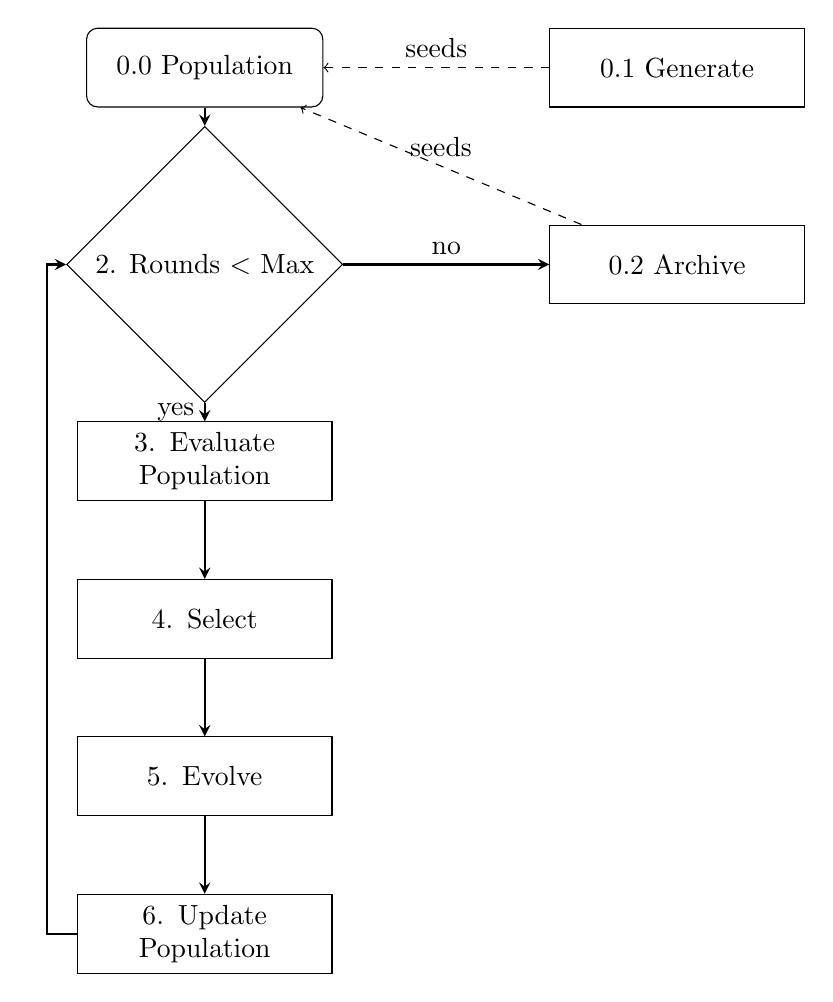
\begin{tikzpicture}[node distance=2cm]
\node (init) [startstop] {0.0 Population};
\node (gen) [process, right of=init, xshift=4cm] {0.1 Generate};
\node (while) [decision, below of=init, yshift=-0.5cm] {2. Rounds $<$ Max};
\node (eval) [process, below of=while, yshift=-0.5cm] {3. Evaluate Population};
\node (select) [process, below of=eval] {4. Select};
\node (evolve) [process, below of=select] {5. Evolve};
\node (update) [process, below of=evolve] {6. Update Population};
\node (archive) [process, right of=while, xshift=4cm] {0.2 Archive};

\draw [arrow] (init) -- (while);
\draw [arrow] (while) -- node[anchor=east]{yes}(eval);
\draw [arrow] (while) -- node[anchor=south]{no}(archive);
\draw [arrow] (eval) -- (select);
\draw [arrow] (select) -- (evolve);
\draw [arrow] (evolve) -- (update);
\draw [dashed, ->] (gen) -- node[anchor=south]{seeds}(init);
\draw [dashed, ->] (archive) -- node[anchor=south]{seeds}(init);

% \draw [arrow] (update) -- (eval);
\draw [arrow] (update)-- +(-2,0) |- (while) node[near start,sloped,above] {};
%\draw [dashed, ->] (update)-- +(+2,0) |- (archive) node[near start,sloped,above] {};
%\draw [dashed, ->] (archive)-- +(0,+1) |- (init) node[near start,sloped,above] {};
\end{tikzpicture}
\\


\paragraph{Datastructures}
The population is kept in a sorted collection with O(1) random access and O(log N) insertion/addition complexity. 

\paragraph{Control flow}
The algorithm performs k runs, each run consists of j generations comprised of the following stages:

\subparagraph{Selection}
Select given a criteria k of the population to modify. The current implementation works on the entire population, this can be easily tuned to select only the k best specimens.

\subparagraph{Evolution}
In the evolution stage 2 operators modify the selected set of specimens.
Mutation will generate a modified specimen which replaces the original based on the fitness score.
Crossover will select 2 specimens and exchange subtrees randomly chosen between the two specimens. The best 2 specimens of the resulting set of 4 are then retained.

\subparagraph{Update}
In the update stage a validation check is done on the new specimens, the modified specimens are added to the population and if needed new specimens are generated.

\subparagraph{Statistics}
At the end of a generation statistics are gathered and stored. The fitness scores and their evolution is tracked for later analysis.
The algorithm can use these to detect stalling convergence.
The entire set of statistics allow for a perfect trace of the algorithm stage by stage.

\subparagraph{Archive}
At the end of a run a selection of the surviving population is stored in the archive. 
The population is then emptied and reseeded using the archive and random specimens. The combination of these approaches ensures the best results of the previous generations are not lost, while introducing new information into the process.


\subsection{Fitness function}
A wide range of fitness functions is possible, in this project a distance function is used that evaluates the tree on a sample of the domain and compares the result with the expected output. 
Several options are available as distance function, the current implementation uses a root mean square. Experiments with a normalized variant and Pearson correlation coefficient are planned. 

\subsection{Complexity}
A complexity measure is implemented based on the operator complexity and depth of the tree. Functions are ordered by complexity giving a higher weight to $\tanh$ compared to $+$. The idea behind this is that a complex function such as $\tanh$, while more expressive, will lead to overfitting more easily than a simpler function. The complexity score is a ratio of the current complexity of all nodes compared to the maximum complexity the tree could have given its depth. This ratio (within [1,2]) is used as a multiplier for the fitness score to influence the algorithm. 

\subsection{Initialization}
Initialization requires constructing a population of expression trees. In a random directed search algorithm this is a random process, but the generation of a random tree can easily generate an invalid tree. Consider a function node with division as operator. It is clear that the right subtree of such a node should never evaluate to zero. 
Several approaches in literature exist %todo ref 
to solve this problem.
As the depth of the tree grows, the complexity of this problem grows exponentially.
The problem is split into detection and remediation.
To detect an invalid tree requires full knowledge of the domain the tree represent. Even if we have this domain, it is not feasible to validate the tree for the entire domain. 
Invalid function input is caught in Python by way of exceptions. 
Exceptions are only justified in high performance code if the probability of an exception is very low. 
It is clear that this is not the case, as the depth of the tree grows the probability of invalid input for a single node grows exponentially. To address this any function node that is invalid will return None to signal an invalid domain.
A naive approach then constructs an entire tree and evaluates it on the domain. 
With the increasing propability of invalid nodes as the depth of the tree increase, this becomes quickly infeasible.
We can constrict the domain to a few values to test at construction. 
Should other values invalidate the tree, the corresponding fitness score will result in the elimination of the tree.
We find thus a balance between generation of semantically correct trees and computational cost. 
It is not feasible to delay all validation to the algorithm itself, this simply moves the naive approach to the algorithm loop.
Finally, by constructing and validating a tree from the bottom up, we can detect early when a tree is invalid. 
In contrast with a top down approach this allows us to recover from invalid choices in the random process without discarding valid subtrees.
The initialization stage is repeated in the algorithm itself at a smaller scale when generating subtrees for the mutation operator and when reseeding the algorithm for a new run.

\subsection{Operators}
The GP algorithm features 2 operators.
\subsubsection{Mutation}
Mutation operates on a single specimen and modifies its structure. Typically a random subtree is chosen, removed and replaced with a newly generated subtree. 
This operation is, depending on the depth of the subtree and the problem domain, expensive as the newly generated subtree has to result in a valid outcome. The same bottom up construction from the initialization code is reused here as a compromise between validity of the specimen and performance.
\paragraph{Configuration}
The mutation operator can be configured to keep the depth of the tree equal. This prevents bloating but also potentially restricts the search space.
Other configurations allow unrestricted growth, or variable growth but limited by a preset value. Experiments are underway to observe the effect on convergence.
Mutation is very invasive, if a large subtree is selected (selection is a random process), a fit specimen can lose most of its value.
Similar to the approach in Simulated Annealing, we can use a target depth configuration that forces mutation to make small changes in highly fit individuals and large in unfit individuals as a perfect balance.
The current implementation mutates only on the lesser fit specimens in the population at an observed increase in runtime without losing fitness.
A mutated specimen replaces its original depending on its fitness.

\subsubsection{Crossover}
Two specimens are selected and copied. Each of the copies exchanges a randomly chosen subtree with the other. This exchange of information leads quickly to convergence, but does not introduce new information (e.g. diversity). 
\paragraph{Configuration}
Crossover can be configured to preserve depth by exchanging subtrees of equal depth. The same concept of modifying highly fit individuals to a smaller extent than less fit individuals can be applied here but with caution, the fitness of the subtree is higher than that of a randomly generated as is the case with mutation.
Crossover in the current implementation picks random pairs of specimens, and from the resulting 4 specimens (2 parents, 2 offspring) picks the 2 best to replace the parents depending on fitness.

\subsection{Constants}
% Demonstrate effect of varying limits of constant generation

\subsection{Parameters}
The algorithm has several key parameters. We will list each and detail the challenges in finding an optimal value.
\begin{itemize}
\item population size : A balance between maximizing diversity and information versus optimal fitness requires different optimal population sizing for each problem instance. 
\item Operator configuration : The operators can restrict bloating by preventing specimens from growing beyond a set limit. The key question remains what the exact valid limit is, and if this excludes optimal solutions from being found.
\item depth limit : The algorithm can force each specimen to maintain a set depth. As before with the operators, this value is at most trial and error. A rule of thumb is to set this value so that at each feature can be present in a leaf in the tree. E.g. with 16 features, depth should be greater or equal to 4. Too large a value will lead to an exponential increase in memory and runtime. Especially validating specimens will become prohibitively expensive.
\item Constant ranges: The bounds for the generated constants influence the algorithm greatly. A small range allows for fast execution but risks losing optimal solutions. A large value leads to high variance in fitness values. 
\item PRNG: the random process and distribution has a significant effect in all stages of the algorithm. For the moment a uniform distribution is used, but experiments are planned with other distributions such a Levy Flight.
\item Generations : A simple problem instance will convergence in very few generations, although this also depends on the population size. More intractable problems require more generations. The optimal value is not known in advance, but the algorithm will detect convergence stalling so picking a large value is preferred.
\item Runs: From the analysis we clearly see that rerunning the algorithm with an archive of previous generations has a benefit on convergence and quality of solutions. New information is introduced while maintaining the best solutions of the previous runs. There is no ideal values for this parameter, but a similar convergence detection as used with the generations is planned. A higher value will then be preferred.
\end{itemize}
%Configure the algorithm how ?
\section{Visualization and Tracing}
Each specimen in the population can be inspected by plotting it as a .dot file. Viewing such a tree in svg format allows for quick insights into how the operators work, how the tree is balanced and how it evolves during the algorithm.
The convergence statistics gathered during execution can be displayed in interactive plots. This is vital for the analysis of the algorithm, especially the convergence over time and the effect of parameter configuration.
Debugging and introspection of a probabilistic search algorithm is notoriously hard. To alleviate this each functioncall can be decorated with a logger, enabling a full blown trace of the entire algorithm. The code itself requires no changes to enable this, simply configuring the right logging object and level is enough.
\section{Analysis of results}

\section{Open Issues}
\subsection{Parameter configuration}
It is clear from the results that configuring the algorithm itself requires tuning of optimal parameters. The domain and samples taken from the domain are defining for the results, as are the generations, runs and other parameters involved. It is hard to estimate these values in advance, but the code
has been extended with checks to make this process easier. For instance convergence detection is present, if the convergence stalls during k generations the current run is halted and a new begun.
\subsection{Complexity measure and Pareto Front}
Defining a 'good' complexity measure is still a work in progress. A balance has to be found between computational complexity (e.g. depth of the tree) and the resulting behavior of the tree (e.g. tendency to over and underfitting)
\subsection{Planning}
The project is on schedule, the last weeks of November saw a delay due to other projects, but this has been made up.
The current phase is nearly concluded : implementation and analysis of a baseline GP algorithm with benchmarks
The next phase starts after the examn period : implementation and integration of a selection of metaheuristic algorithms.
\section{Supporting Code}
\subsection{Testing}
Extensive tests are available guaranteeing correctness of each part of the project. 
Considering the probabilistic nature of the algorithms this is required to ensure the results are valid and deterministic (if given a seed).
This also means that results are reproducible, vital for the analysis and conclusions.
\subsection{Expressions}
Conversion functions were written to enable parsing expressions from and to tree forms, including but not limited to a simple expression parser and tokenizer, and a number of utility functions.
\subsection{Visualization}
The expression trees can be written out to .dot format. Such a graphic visualization has proven to be invaluable in debugging the code as well as analyzing the behavior of the algorithm. The statistics gathered during the execution of the algorithm are output as interactive plots. This representation allows analysis of the convergence of the algorithm in time. This functionality will become even more useful in the remainder of the project.
\subsection{Constants}
To make the integration of the metaheuristic optimizers easier, the design has integrated a set of accessors retrieving all Constant objects from an expression tree in vector form. This provides the optimization algorithm a quick interface to the tree structure.
\bibliography{papers}
\end{document}